\chapter{Conception et implémentation de l’application}

\section{Conception}

\subsection{Introduction}
Tout comme la construction d’une maison nécessite des plans à différents niveaux (vision extérieure, plan des différents étages, plans techniques…), la réalisation d’une application informatique ou d’un ensemble d’applications est basée sur plusieurs diagrammes. Ces diagrammes doivent unifier la vision de l’équipe de développement et l’orienter vers la création d’une solution bien alignée sur les exigences du problème, et permettre également à l’équipe de proposer à ses clients une expérience utilisateur cohérente tout au long de l’application. 

Pour atteindre l'objectif de communiquer une vision ou un système difficile à expliquer par des mots, différents langages de modélisation ont été créés, tels que SysML, BON et le langage \acrshort{UML} le plus connu et le plus utilisé, ainsi que des méthodes anciennes et récentes, telles que le wireframing.

La pratique des conceptions logicielles n’est pas une pratique rigide dans laquelle plusieurs étapes clés sont toujours présentes dans un ordre particulier, par exemple : Le langage UML ne préconise aucune démarche, ce n’est donc pas une méthode. Chacun est libre d’utiliser les types de diagramme qu’il souhaite, dans l’ordre qu’il veut. Il suffit que les diagrammes réalisés soient cohérents entre eux, avant de passer à la réalisation du logiciel.

\subsection{Diagrammes de base}
\subsubsection{Diagrammes de séquence}

\begin{figure}[h]
	\begin{center}
		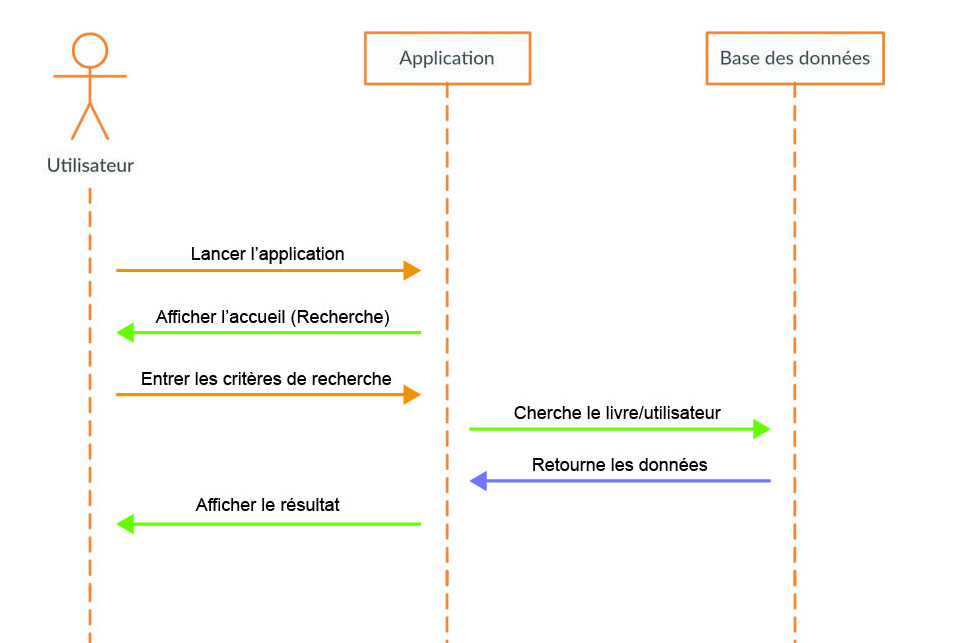
\includegraphics[width=8cm]{Images/chapter3/rechercher_un_livre.jpg}
		\caption{{\footnotesize l'enchaînement des actions pour la recherche d'un  livre particulier}}
	\end{center}
\end{figure}

\begin{figure}[h]
	\begin{center}
		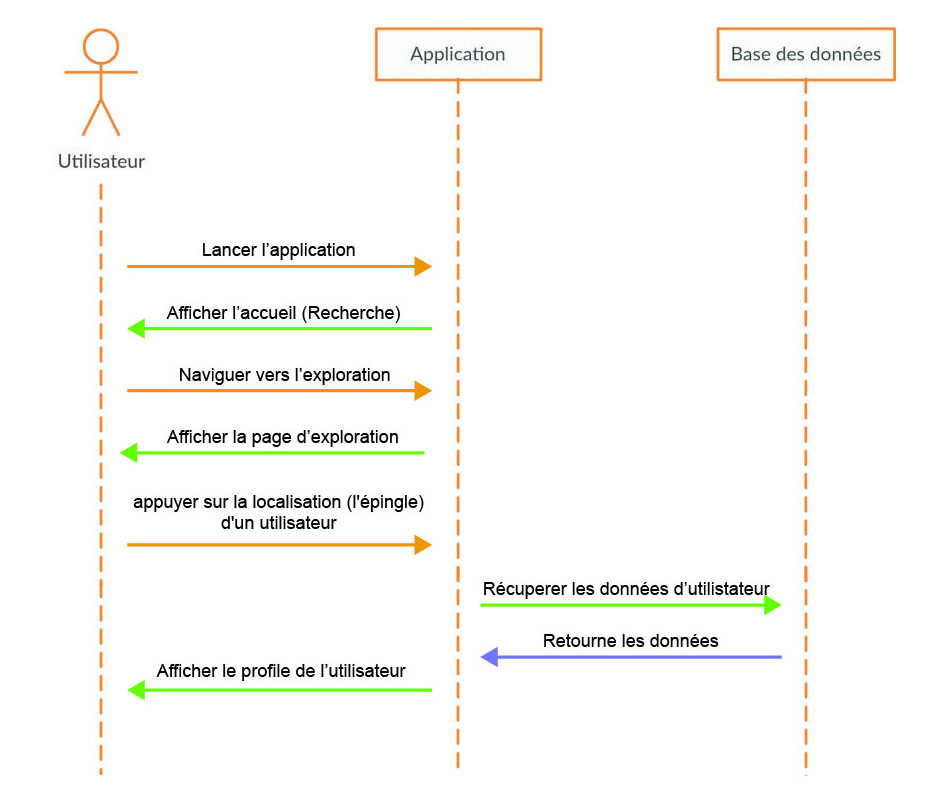
\includegraphics[width=8cm]{Images/chapter3/explorer_les_livres.jpg}
		\caption{{\footnotesize l'exploration des livres/utilisateurs à proximité}}
	\end{center}
\end{figure}

\newpage

\subsubsection{Diagramme de navigation}

\begin{figure}[h]
	\begin{center}
		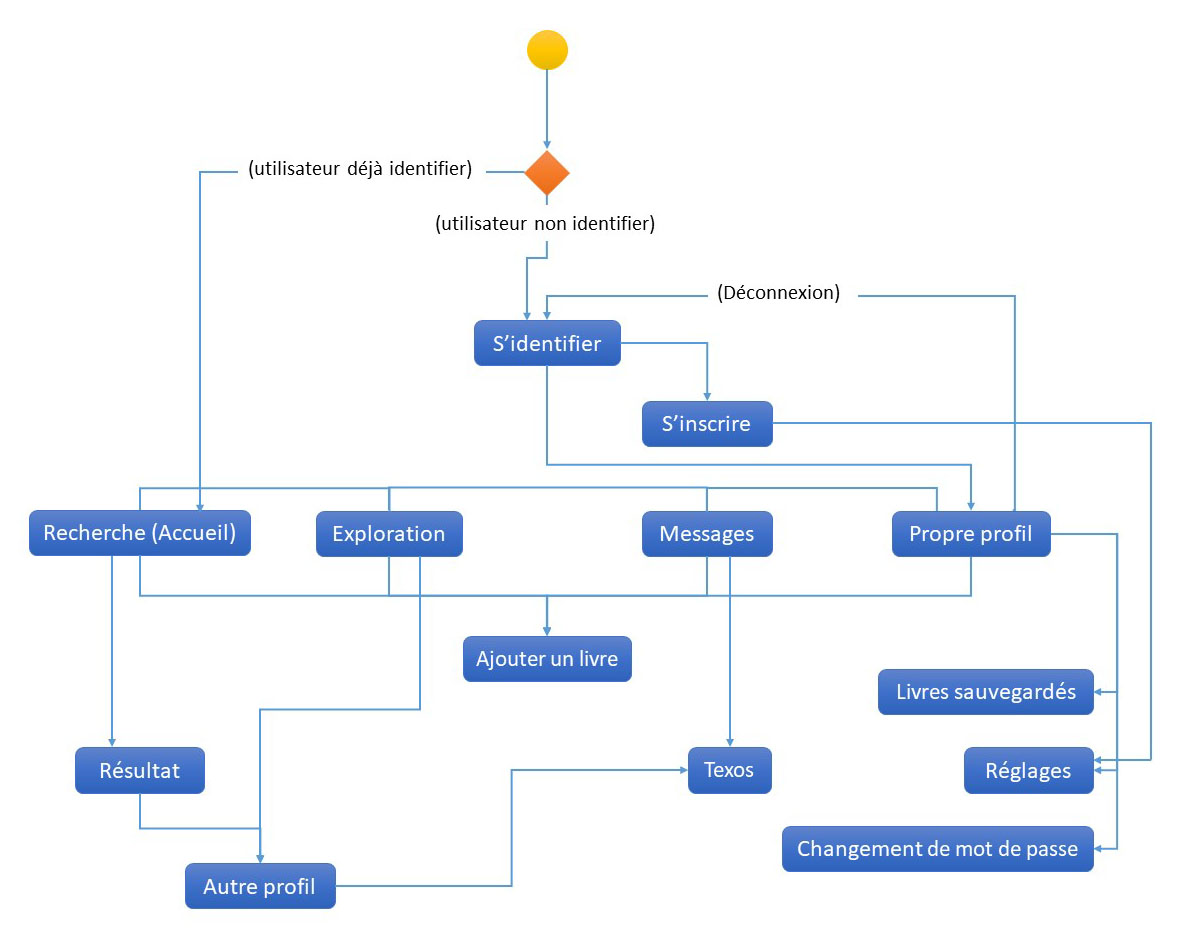
\includegraphics[width=14cm]{Images/chapter3/diagramme_de_navigation.jpg}
		\caption{{\footnotesize l'architecture de navigation}}
	\end{center}
\end{figure}

\subsection{Maquette fonctionnelle (Wireframe)}
Le wireframe ou maquette fonctionnelle est un schéma utilisé lors de la conception d'une interface pour définir les zones et composants qu'elle doit contenir. À partir d'un wireframe peut être réalisée l'interface proprement dite par un graphiste. La démarche de recourir à des wireframes s'inscrit dans une recherche d'ergonomie. Elle est surtout utilisée dans le cadre du développement logiciel et des sites et applications Web. Le wireframe consiste concrètement en un croquis, un collage papier ou un schéma numérique\cite{noauthor_wireframe_nodate}.




\section{Implémentation}
